% Options here are passed to the article class.
% Most common options: 10pt, 11pt, 12pt
\documentclass[10pt]{datasheet}

% Input encoding and typographical rules for English language
\usepackage[utf8]{inputenc}
\usepackage[english]{babel}
\usepackage[english]{isodate}

% tikz is used to draw images in this example, but you can
% also use \includegraphics{}.
\usepackage{graphicx}

% These define global texts that are used in headers and titles.
\title{SG01: Shulker Box Splitter Array}
\author{Quacon Group}
\tags{splitting}
\date{21 December 2022}
\revision{Revision 2}
\begin{document}
\maketitle

\section{Features}

\begin{itemize}
\item{No "filter items"}
\item{2 wide tileable design}
\end{itemize}

\section{Applications}

\begin{itemize}
\item{Dynamic sorting systems}
\end{itemize}

\section{General Description}
Splits mixed boxes into smaller boxes of the same type. This design uses the hopper dueling mechanism for a "filter itemless" setup. Video explanation \href{https://www.youtube.com/watch?v=zRO1QfmYa6o}{here}.
\vfill\break

\begin{figure}[h]
    \centering
    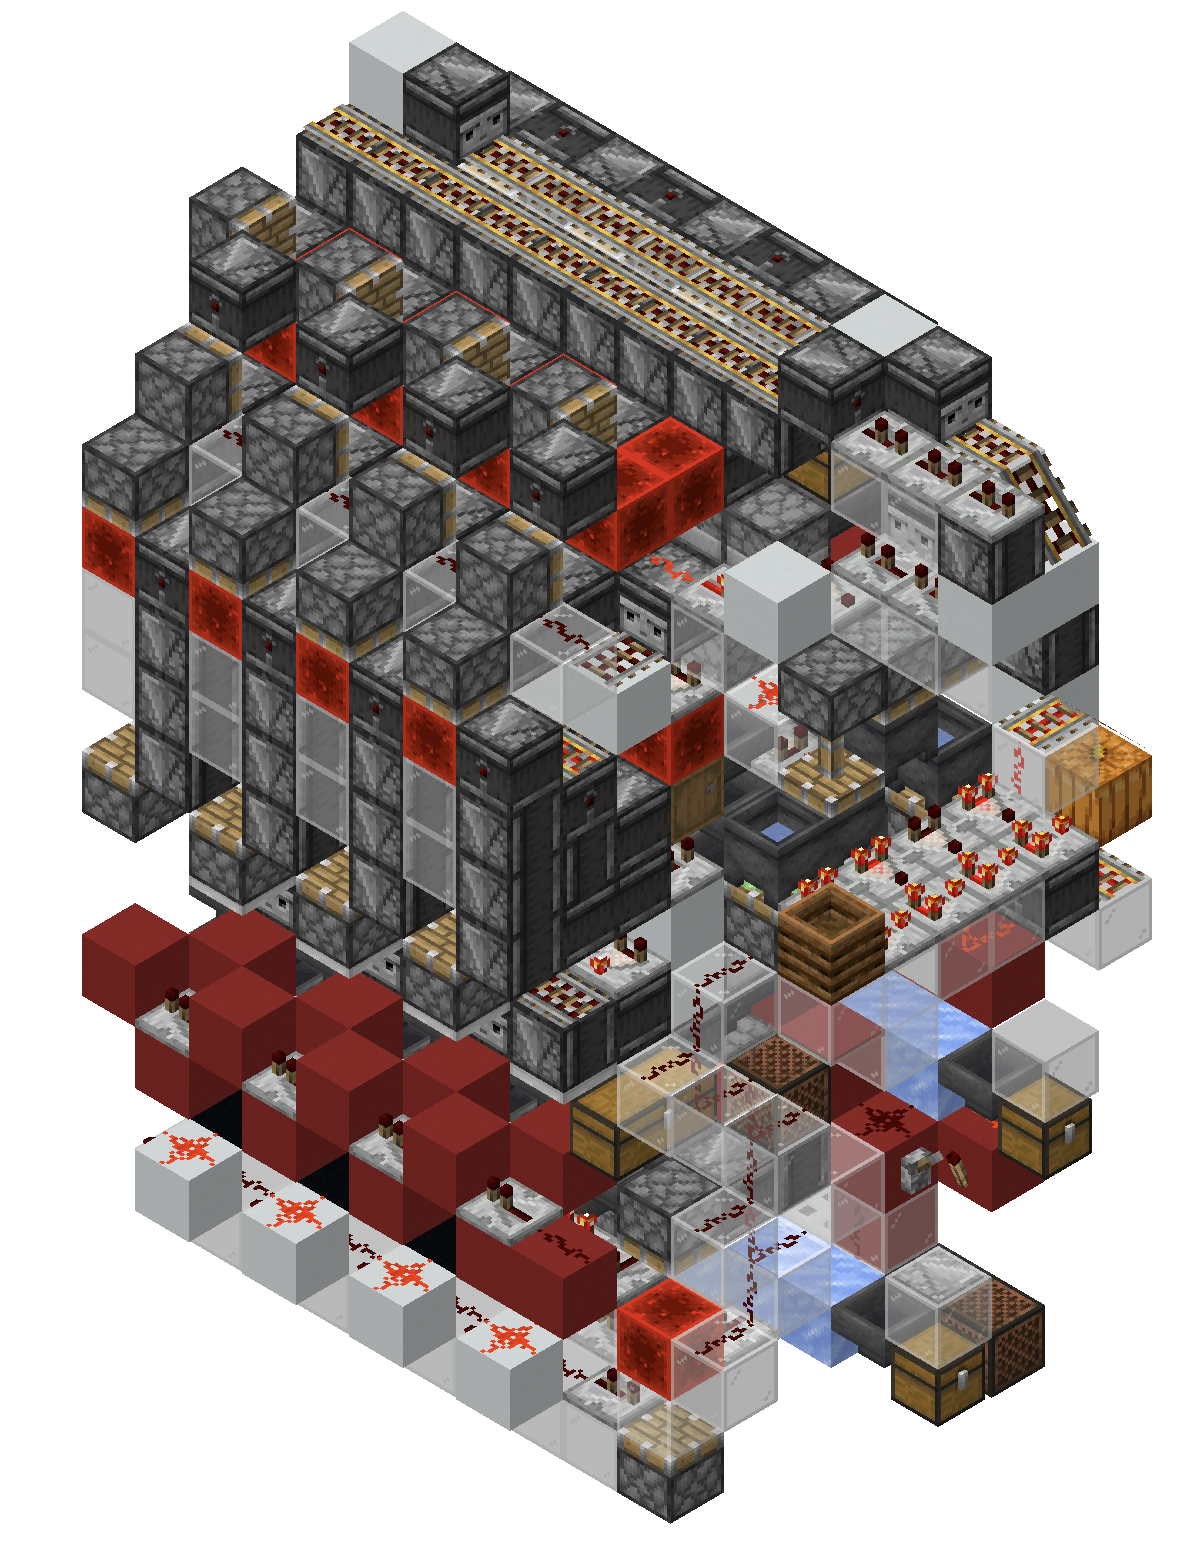
\includegraphics[width=0.48\textwidth]{splitarray.png}
    \caption{\centering Shulker Box Splitter Array}
\end{figure}

% For wide tables, a single column layout is better. It can be switched
% page-by-page.
\onecolumn

\section{Device Specifications}

\begin{table}[h]
    \caption{Inputs}
    \begin{tabularx}{\textwidth}{l | c | X}
        \thickhline
        \textbf{Name} & \textbf{Range} & \textbf{Description} \\
        \hline
        Mixed boxes input & Box & Boxes to split. Boxes can contain any items. \\
        \thickhline
\end{tabularx}
\end{table}

\begin{table}[h]
    \caption{Outputs}
    \begin{tabularx}{\textwidth}{l | c | X}
        \thickhline
        \textbf{Name} & \textbf{Range} & \textbf{Description} \\
        \hline
        Split boxes output & Box & Boxes with same item types only \\
        \hline
        Unstackables output & Item & Unstackable items \\
        \thickhline
\end{tabularx}
\end{table}

\begin{table}[h]
    \caption{Device Specifications}
    \begin{tabularx}{\textwidth}{l | c c c | c | X}
        \thickhline
        \textbf{Parameter} & \textbf{Min.} & \textbf{Typ.} & \textbf{Max.} &
        \textbf{Unit} & \textbf{Conditions} \\
        \hline
        MC Version & 1.16.5 & 1.16.5 & - & MCV & Latest version at time of writing: 1.19.3\\
        \hline
        Dimensions & & 14 x 19 x 9 & & Blocks & \\
        \thickhline
\end{tabularx}
\end{table}
\newpage
\section{Testing Data}
\begin{table}[h]
\caption{Executed Tests}
\begin{tabularx}{\textwidth}{l | X}
    \thickhline
    \textbf{Test} & \textbf{Result} \\
    \hline
    Splitting test & Device was able to split mixed boxes correctly. \\
    \thickhline
\end{tabularx}
\end{table}

\section{Download Information}
\begin{table}[h]
    \caption{Download Information}
    \begin{tabularx}{\textwidth}{l | l | l | X}
        \thickhline
        \textbf{Identifier} & \textbf{MC} & \textbf{File} & \textbf{Description} \\
        \hline
        SG01 & 1.17.1 & \href{https://github.com/Soontech-Annals/Archive/blob/364bde8dbcbc2e5337489ff435bcda9b387017e2/Archive/splitting/SG01\%20Shulker\%20Box\%20Splitter\%20Array/SG01\_Shulker\_Box\_Splitter\_Array.zip?raw=1}{SG01\_Shulker\_Box\_Splitter\_Array.zip} & World download of device. \\
        \hline
        \thickhline
    \end{tabularx}
\end{table}

\end{document}

